\begin{figure}[H]
\begin{tabular}{@{}c@{}c@{}c@{}}
\begin{subfigure}[b]{0.30\textwidth}
\begin{center}
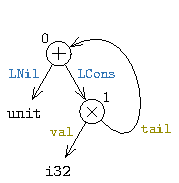
\includegraphics[scale=1.3]{chapters/figures/figTypeTreeList1.pdf}
\end{center}
\vspace{30px}
\caption{\label{fig:typetreelistpeel1} Canonical \type{List} ADT}
\end{subfigure}%
&
\begin{subfigure}[b]{0.33\textwidth}
\begin{center}
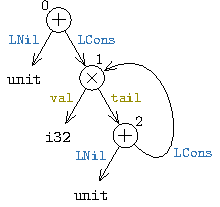
\includegraphics[scale=1.3]{chapters/figures/figTypeTreeList2.pdf}
\end{center}
\vspace{20px}
\caption{\label{fig:typetreelistpeel2} Peeled \type{List} ADT}
\end{subfigure}%
&
\begin{subfigure}[b]{0.33\textwidth}
\begin{center}
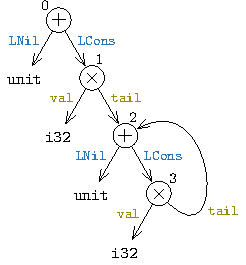
\includegraphics[scale=1.3]{chapters/figures/figTypeTreeList3.pdf}
\end{center}
\caption{\label{fig:typetreelistpeel3} Unrolled \type{List} ADT}
\end{subfigure}%
\\
\end{tabular}
\caption{\label{fig:typetreespeel}Three equivalent graphical representations for \type{List} ADT.
\Cref{fig:typetreelistpeel1} shows the graphical representation of the canonical form of \type{List}.
\Cref{fig:typetreelistpeel2} is obtained by peeling the {\em backedge} [2,1] in \cref{fig:typetreelistpeel1}.
\Cref{fig:typetreelistpeel3} is obtained by unrolling the backedge [2,1] in \cref{fig:typetreelistpeel1} or by
peeling the backedge [4,1] in \cref{fig:typetreelistpeel2} respectively.}
\end{figure}